% Uncomment this to make slides with overlays:
%\documentclass[slides]{beamer}

% Uncomment these (but comment the above \documentclass line) to make handouts:
\documentclass[handout]{beamer}

% Uncomment these to have more than one slide per page
\usepackage{pgfpages}
\pgfpagesuselayout{2 on 1}[border shrink=5mm]
\pgfpageslogicalpageoptions{1}{border code=\pgfusepath{stroke}}
\pgfpageslogicalpageoptions{2}{border code=\pgfusepath{stroke}}

\usepackage[]{graphicx, color, hyperref}

\mode<presentation>
{
	%\usetheme[secheader]{Boadilla}
	%\usecolortheme[rgb={.835, .102,.169}]{structure}  
	\usetheme[width= 0cm]{Goettingen}
	%\setbeamercovered{transparent}
}
\setbeamertemplate{navigation symbols}{}
\setbeamertemplate{footline}[frame number]

\definecolor{blue2}{rgb}{0.278,0.278,0.729} 
\newcommand{\blue}[1]{\textcolor{blue2}{#1}}
\newcommand{\white}[1]{\textcolor{white}{#1}}
\newcommand{\red}[1]{\textcolor{red}{#1}}
\newcommand{\xbar}{\overline{x}}
\newcommand{\ybar}{\overline{y}}
\newcommand{\phat}{\widehat{p}}
\newcommand{\prob}{\mbox{Pr}}
\newcommand{\E}{\mathbb{E}}
\newcommand{\Var}{\mbox{Var}}
\newcommand{\cp}{\oplus}
\newcommand{\cm}{\circleddash}


\title{Lecture 29: Expected Value and Variance}
\author{Chapter 2.4}
\date{}


\begin{document}
%------------------------------------------------------------------------------
\begin{frame}
\titlepage
\end{frame}
%------------------------------------------------------------------------------


%------------------------------------------------------------------------------
\begin{frame}[fragile]
\frametitle{Random Variable}

%
% Comment this
%
%A random process or variable with a numerical outcome is called a \blue{random variable}, and is typically denoted by an upper case letter.  E.g. $X, Y, \mbox{or } Z$

\end{frame}
%------------------------------------------------------------------------------


%-------------------------------------------------------------------------------
\begin{frame}
\frametitle{Intuitively Thinking: Expected Value}
 
%
% Comment this
% 
%Easy example:  Coin flips.  Say we flip a fair coin $n=10$ times with probability $p=\frac{1}{2}$ of heads.
%
%\pause
%\vspace{0.5cm}
%
%How many heads do you \blue{expect} to get?
%
%\vspace{0.5cm}
%
%$n \times p = 10 \times \frac{1}{2} = 5$

\end{frame}
%-------------------------------------------------------------------------------


%x <- c(2, 3, 4, 10, 11)
%fx <- c(3,5,2,6,4)
%fx <- fx/sum(fx)
%
%pdf("./4.1 Discrete Expectation/mean.pdf", width=8, height=5)
%plot(x, fx, ylab="f(x)", ylim=c(0, max(fx)))
%points(x, fx, pch=19, cex=1.5)
%for(i in 1:5)
%  lines(c(x[i], x[i]), c(0, fx[i]), lwd=5)
%
%mu <- sum(x*fx)
%abline(h=0)
%title(sprintf("Mean = %4.2f", mu))
%points(mu, 0, col="red", pch=19, cex=2)
%dev.off()
%
%library(xtable)
%xtable(data.frame(rbind(x, fx)))
%-------------------------------------------------------------------------------
\begin{frame}
\frametitle{Intuitively Thinking: Expected Value}
Say you have a random variable $X$:
\begin{center}
\begin{tabular}{r|ccccc}
  \hline
$x$ & 2 & 3 & 4 & 10 & 11 \\ 
  $\prob(X=x)$ & $\frac{15}{100}$ & $\frac{25}{100}$ & $\frac{10}{100}$ & $\frac{30}{100}$ & $\frac{20}{100}$\\ 
   \hline
\end{tabular}
\end{center}

\vspace{0.5cm}

E.g. We observe $X=3$ with prob .25

\pause
\vspace{0.5cm}

\pause Is the value we expect to observe: 
\begin{eqnarray*}
\frac{2 + 3 + 4 + 10 + 11}{5} &=& 6 \mbox{ ?}
\end{eqnarray*}

\end{frame}
%-------------------------------------------------------------------------------


%-------------------------------------------------------------------------------
\begin{frame}
\frametitle{Intuitively Thinking: Expected Value}
No, each of the $x$'s have different \blue{probability} of occurring.

\vspace{0.25cm}

\pause
For each $x$, we assign different \blue{weights} $\prob(X=x)$ and not $\frac{1}{5}$:

\begin{eqnarray*}
2 \times \frac{15}{100} + 3 \times \frac{25}{100} + 4 \times \frac{10}{100} + 10 \times \frac{30}{100} + 11 \times \frac{20}{100} = 6.65
\end{eqnarray*}

\end{frame}
%-------------------------------------------------------------------------------


%-------------------------------------------------------------------------------
\begin{frame}
\frametitle{Expected Value}
%
% Comment this
%
%The \blue{expected value} is a \blue{weighted average} of all possible values $x$.  This can be thought of as a measure of \blue{center}:
%\[
%\E[X] = \sum_{i=1}^k x_i \cdot \prob(X=x_i) 
%\]
%
%This is also called the \blue{mean} and \blue{expectation} of $X$.  Typically denoted by $\mu$.
\end{frame}
%-------------------------------------------------------------------------------


%-------------------------------------------------------------------------------
\begin{frame}
\frametitle{Expected Value}
You can also think of the mean as the \blue{center of mass or balance point}. It is 6.65 (marked with red point):


\begin{center}
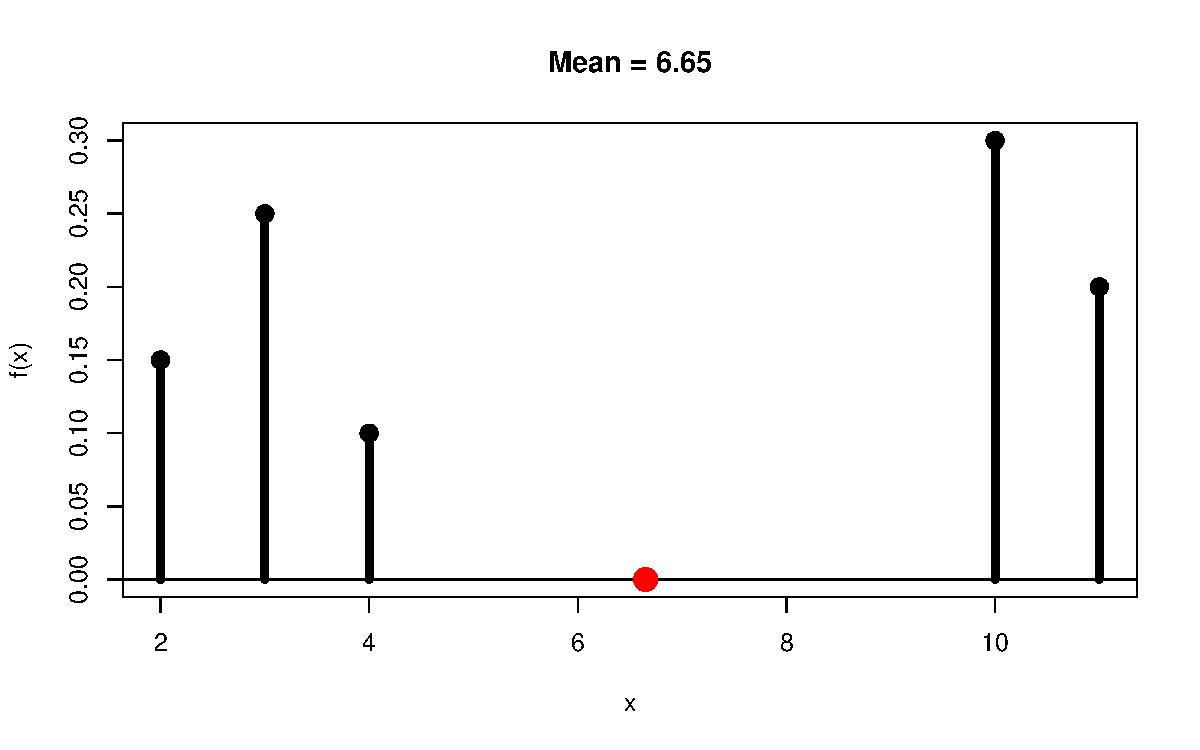
\includegraphics[width=0.7\textwidth]{figure/mean}
\end{center}

\end{frame}
%-------------------------------------------------------------------------------


%pdf("./13.3 Probability Theory/spread.pdf", width=8, height=5)
%x <- seq(-30,30,by=0.05)
%plot(x,dnorm(x,0,5),type='l', ylab="P(X=x)")
%lines(x,dnorm(x,0,10), lty=2, col=2)
%dev.off()
%
%pdf("./13.3 Probability Theory/spread1.pdf", width=8, height=5)
%x <- seq(-30,30,by=0.05)
%fx <- dnorm(x,0,5)
%plot(x, fx, type='l', ylab="P(X=x)", xlim=c(-20, 20))
%dev.off()
%
%pdf("./13.3 Probability Theory/spread2.pdf", width=8, height=5)
%plot(x, fx, type='l', ylab="P(X=x)", xlim=c(-20, 20))
%abline(v=0)
%x1 <- 7
%fx1 <- dnorm(x1, 0, 5)
%points(x1, 0, pch=19, cex=1)
%lines(c(x1,x1), c(0, fx1), lty=2)
%#title(sprintf("x = %2.1f and Deviation from Mean = %2.1f,   f(x) = %2.3f",  x1, x1-0, fx1))
%arrows(0, fx1, x1, fx1, code=3, length=0.1)
%dev.off()
%
%pdf("./13.3 Probability Theory/spread3.pdf", width=8, height=5)
%plot(x, fx, type='l', ylab="P(X=x)", xlim=c(-20, 20))
%abline(v=0)
%x1 <- -3
%fx1 <- dnorm(x1, 0, 5)
%points(x1, 0, pch=19, cex=1)
%lines(c(x1,x1), c(0, fx1), lty=2)
%#title(sprintf("x = %2.1f and Deviation from Mean = %2.1f,   f(x) = %2.3f",  x1, x1-0, fx1))
%arrows(0, fx1, x1, fx1, code=3, length=0.1)
%dev.off()
%
%pdf("./13.3 Probability Theory/spread4.pdf", width=8, height=5)
%plot(x, fx, type='l', ylab="P(X=x)", xlim=c(-20, 20))
%abline(v=0)
%x1 <- 10
%fx1 <- dnorm(x1, 0, 5)
%points(x1, 0, pch=19, cex=1)
%lines(c(x1,x1), c(0, fx1), lty=2)
%#title(sprintf("x = %2.1f and Deviation from Mean = %2.1f,   f(x) = %2.3f",  x1, x1-0, fx1))
%arrows(0, fx1, x1, fx1, code=3, length=0.1)
%dev.off()
%-------------------------------------------------------------------------------
\begin{frame}
\frametitle{Intuitively Thinking:  Measures of Spread}
Consider the following distribution with $\mu=0$.  Let's build a measure of \blue{expected ``spread''}. 
\begin{center}
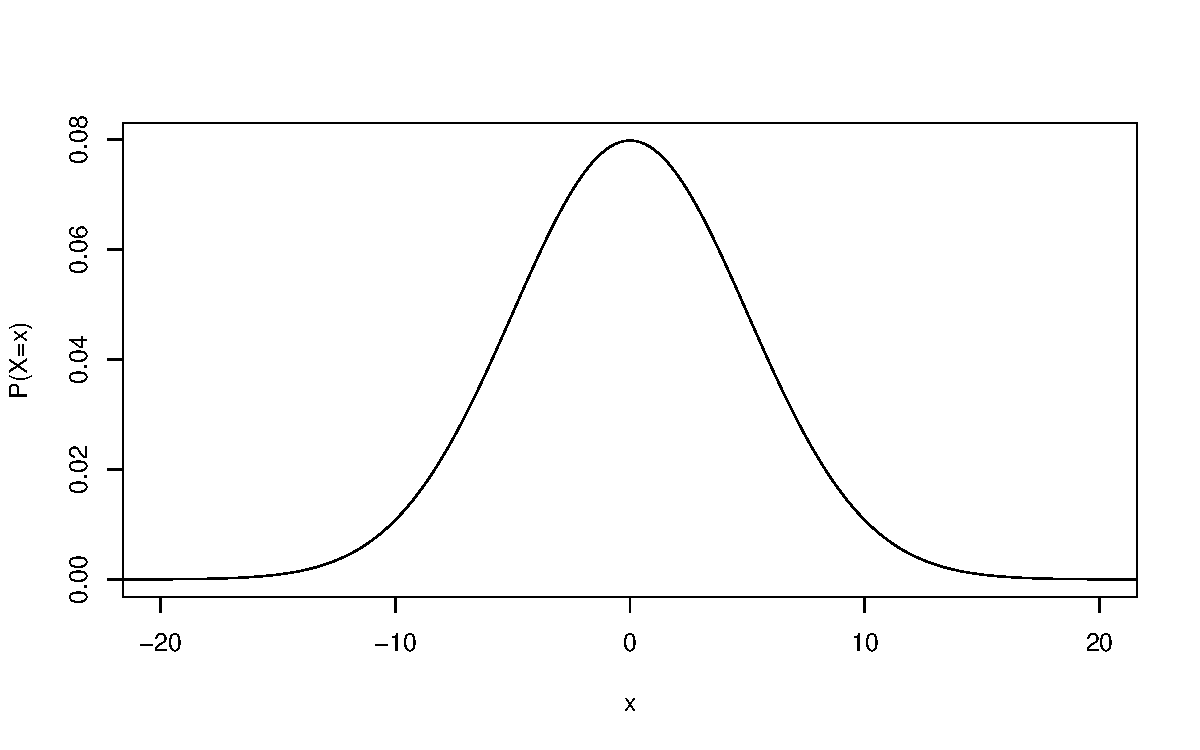
\includegraphics[width=0.7\textwidth]{figure/spread1}
\end{center}
\pause Let's define ``spread'' as the \blue{absolute deviation from $\mu$}: $|x - \mu|$.\\
i.e. $+$'ve \& $-$'ve deviations are treated the same.
\end{frame}
%-------------------------------------------------------------------------------


%-------------------------------------------------------------------------------
\begin{frame}
\frametitle{Intuitively Thinking:  Measures of Spread}
When $x=-3.0$, the abs. deviation from $\mu$ is $|-3.0 - \mu|= 3.0$.\\
Note $P(X=x) = 0.066$.

\begin{center}
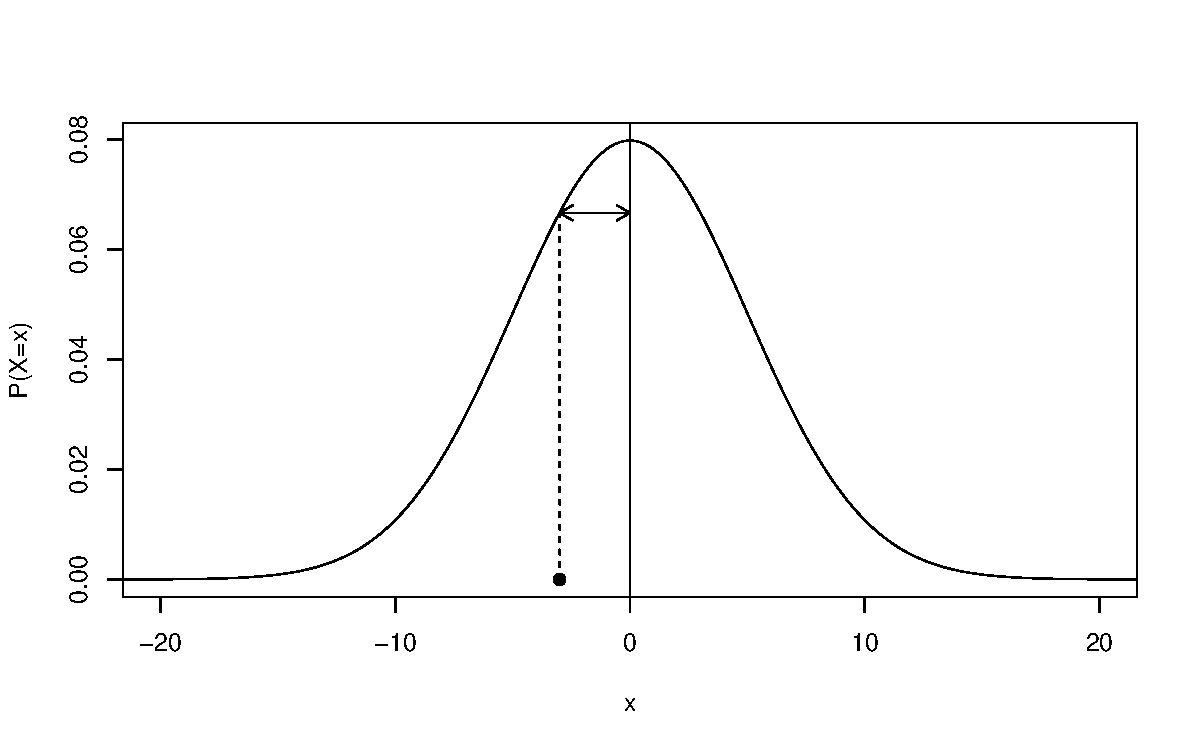
\includegraphics[width=0.7\textwidth]{figure/spread3}
\end{center}

\end{frame}
%-------------------------------------------------------------------------------


%-------------------------------------------------------------------------------
\begin{frame}
\frametitle{Intuitively Thinking:  Measures of Spread}
When $x=7.0$, the abs. deviation from $\mu$ is $|7.0 - \mu| = 7.0$.\\
Note $P(X=x) = 0.030$.

\begin{center}
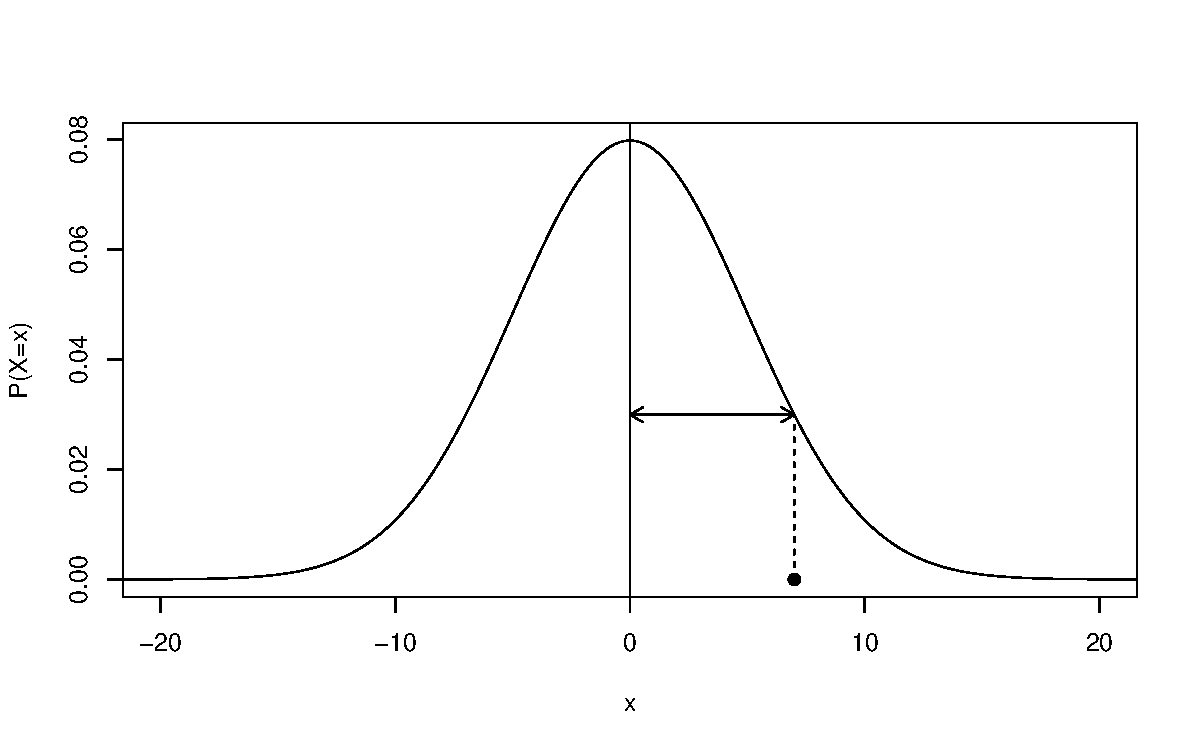
\includegraphics[width=0.7\textwidth]{figure/spread2}
\end{center}

\end{frame}
%-------------------------------------------------------------------------------


%-------------------------------------------------------------------------------
\begin{frame}
\frametitle{Intuitively Thinking:  Measures of Spread}
When $x=10.0$, the abs. deviation from $\mu$ is $|10.0 - \mu| = 10.0$.\\
Note $P(X=x) = 0.011$.

\begin{center}
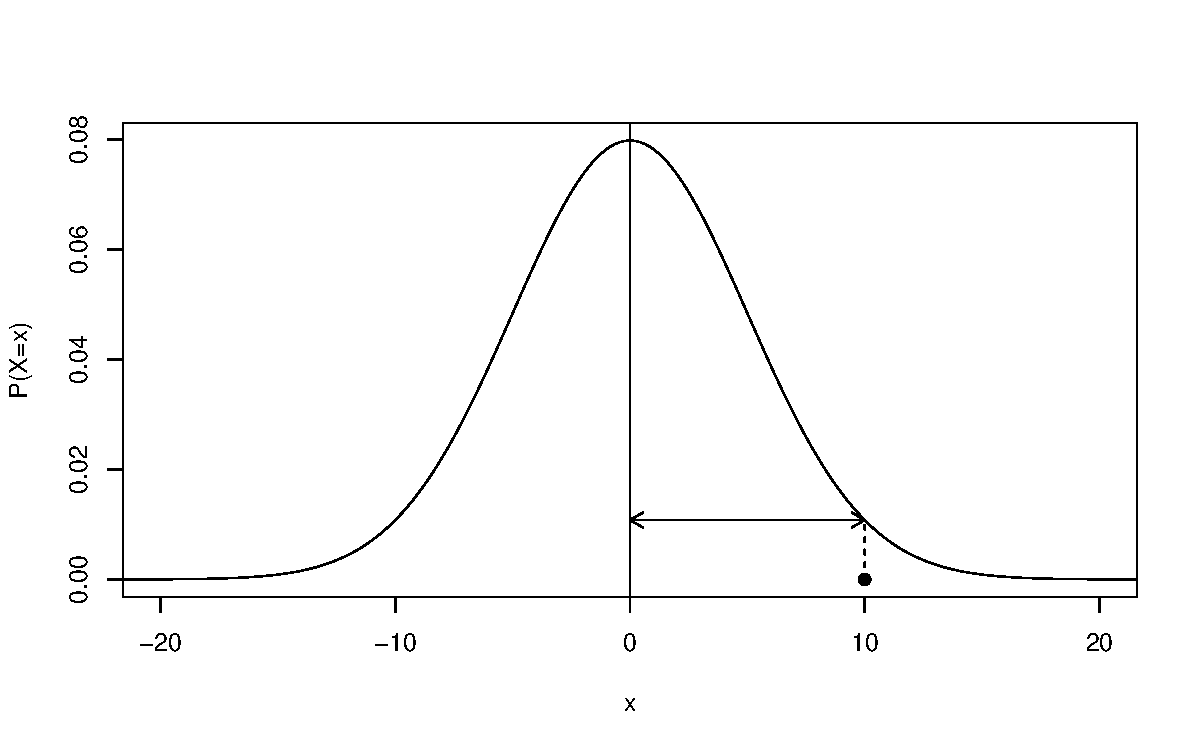
\includegraphics[width=0.7\textwidth]{figure/spread4}
\end{center}

\end{frame}
%-------------------------------------------------------------------------------


%-------------------------------------------------------------------------------
\begin{frame}
\frametitle{Intuitively Thinking:  Measures of Spread}

%
% Comment this
%
\begin{center}
\begin{tabular}{c|cc}
 & Abs Deviation & Weight \\
x& $|x-\mu|$  & $P(X=x)$\\
\hline
-3.0 & $|-3.0 - 0|=3.0$  & 0.066\\
7.0 & $|7.0-0|=7.0$ & 0.030\\
10.0 & $|10.0-0| = 10.0$ & 0.011\\
\end{tabular}
\end{center}

So say we do this for \blue{all} $x$ and take a \blue{weighted average} of the $|x-\mu|$ where the weights are $P(X=x)$.

\vspace{0.5cm}

Voil\`{a}:  Our notion of \blue{expected spread}.  

\end{frame}
%-------------------------------------------------------------------------------


%-------------------------------------------------------------------------------
\begin{frame}
\frametitle{Variance}
%
% Comment this
%
%The variance $\sigma^2$ AKA Var(X) of a distribution is
%\begin{eqnarray*}
%\E\left[(X-\mu)^2\right] = \sum_{i=1}^k (x_i-\mu)^2 \cdot P(X=x_i)
%\end{eqnarray*}
%
%\pause\vspace{0.5cm}
%
%It is the expected \blue{squared} deviation from the mean, and not \blue{absolute} deviation (like in our example).  i.e. not
%\begin{eqnarray*}
%\E\left[|X-\mu|\right] = \sum_{i=1}^k |x_i-\mu| \cdot P(X=x_i)
%\end{eqnarray*}
%
%\pause \vspace{0.5cm}
%Why square?  Treats $+$'ve and $-$'ve deviations as the same, but also easier to do calculus on $x^2$ than $|x|$.

\end{frame}
%-------------------------------------------------------------------------------


%-------------------------------------------------------------------------------
\begin{frame}
\frametitle{Estimators}

%
% Comment this
%
%$\xbar$ is a point \textit{estimate} of $\mu$.   $\xbar$ is based on \blue{observed data}.
%
%\pause
%\vspace{0.25cm}
%
%Before we've observed the data, $\overline{X}$ is still random and is the \textit{estimator} of $\mu$.

\end{frame}
%-------------------------------------------------------------------------------


%-------------------------------------------------------------------------------
\begin{frame}
\frametitle{Sample Mean as an Estimator}

%
% Comment this
%
%So whereas, for a single $X$
%\begin{itemize}
%\item $\E[X] = \mu$
%\item $\Var[X] = \sigma^2$
%\end{itemize}
%
%\vspace{0.25cm}
%
%\pause we have for $\overline{X}$
%
%\vspace{0.25cm}
%
%\begin{itemize}
%\item $\E\left[ \ \overline{X} \ \right] = \mu$
%\item $\Var\left[ \ \overline{X} \ \right] = \frac{\sigma^2}{n}$
%\end{itemize}
%i.e. as $n \longrightarrow \infty$ the variance goes to 0.  

\end{frame}
%-------------------------------------------------------------------------------


%%-------------------------------------------------------------------------------
%\begin{frame}
%\frametitle{Bias}
%
%%
%% Comment this
%%
%One property we want our estimators to have is \blue{unbiasedness}.  i.e.
%
%\begin{eqnarray*}
%\E[\widehat{\theta} - \theta] = 0 &\Rightarrow & \E[\widehat{\theta}] = \theta
%\end{eqnarray*}
%
%\pause i.e. we expected the estimator's value to be the unknown parameter.  
%
%\end{frame}
%%-------------------------------------------------------------------------------
%
%
%%------------------------------------------------------------------------------
%\begin{frame}
%\frametitle{Recall from Earlier}
%
%One example of a non-representative sample is a \blue{biased sample}. For example, \blue{convenience samples} are samples where individuals who are easily accessible are more likely to be included.  
%
%\end{frame}
%%------------------------------------------------------------------------------
%
%
%%------------------------------------------------------------------------------
%\begin{frame}
%\frametitle{Recall from Earlier}
%
%\begin{small}
%\begin{enumerate}
%\item The Royal Air Force wants to study how resistant their airplanes are to bullets. They study the bullet holes on all the airplanes on the tarmac after an air battle against the Luftwaffe (German Air Force).
%\item I want to know the average income of Reed graduates in the last 10 years.  So I get the records of 10 randomly chosen Reedies.  They all answer and I take the average.
%\item Imagine it's 1993 i.e. almost all households have landlines.  You want to know the average number of people in each household in Portland.  You randomly pick out 500 phone numbers from the phone book and conduct a phone survey.
%\item You want to know the prevalence of illegal downloading of TV shows among Reed students.  You get the emails of 100 randomly chosen Reedies and ask them ``How many times did you download a pirated TV show last week?''
%\end{enumerate}
%\end{small}
%
%\end{frame}
%%------------------------------------------------------------------------------






\end{document}











%------------------------------------------------------------------------------
\begin{frame}
\frametitle{One Last Time}
You have a new hypothesis testing machine.  For any hypothesis test it either concludes:
\begin{itemize}
\item ``reject $H_0$ in favor of $H_A$''.  Call this a $\cp$'ve result
\item ``do not reject $H_0$''.  Call this a $\cm$'ve result.
\end{itemize}
\pause
\vspace{0.5cm}

The machine has the following performance specifications:
\begin{itemize}
\item $\alpha=\prob(\mbox{Reject } H_0 \mbox{ when $H_0$ true}) = \prob(\cp|H_0)$
\item Power $=1-\beta=\prob(\mbox{Reject } H_0 \mbox{ when $H_A$ true}) = \prob(\cp|H_A)$
\end{itemize} 

\end{frame}
%------------------------------------------------------------------------------


%------------------------------------------------------------------------------
\begin{frame}
\frametitle{How Reliable Are Your Test Results?}

\begin{center}
  \begin{tabular}{cc|cc}
     \multicolumn{2}{c}{}  & \multicolumn{2}{c}{\textbf{Test conclusion}} \\ 
     &  & $\cm$ & $\cp$ \\ 
\hline
    \textbf{Truth} & $H_0$ true & True Negative (TN) & False Positive (FP) \\
     & $H_A$ true & False Negative (FN) & True Positive (TP)\\ 
    \hline
  \end{tabular}
\end{center}

\begin{itemize}
\pause\item Of the times that we get $\cp$, the proportion it was right is $\prob(H_A|\cp) = \frac{TP}{TP+FP} = $ \blue{positive predictive value}
\pause\item Of the times that we get $\cm$ the proportion it was right is $\prob(H_0|\cm)$? \ $\frac{TN}{TN+FN} = $ \blue{negative predictive value}.  
\end{itemize}

\end{frame}
%------------------------------------------------------------------------------


%------------------------------------------------------------------------------
\begin{frame}
\frametitle{Related Alternative Measure of Reliability}

\begin{center}
  \begin{tabular}{cc|cc}
     \multicolumn{2}{c}{}  & \multicolumn{2}{c}{\textbf{Test conclusion}} \\ 
     &  & $\cm$ & $\cp$ \\ 
\hline
    \textbf{Truth} & $H_0$ true & True Negative (TN) & False Positive (FP) \\
     & $H_A$ true & False Negative (FN) & True Positive (TP)\\ 
    \hline
  \end{tabular}
\end{center}

\pause The \blue{false discovery rate} FDR is 
\begin{eqnarray*}
\mbox{FDR} &=& \frac{FP}{TP + FP} = \prob(H_0|\cp)\\
\pause &=& 1 -\frac{TP}{TP+FP} = 1 - \mbox{Positive Predictive Value}
\end{eqnarray*}

\end{frame}
%------------------------------------------------------------------------------


%------------------------------------------------------------------------------
\begin{frame}
\frametitle{Multiple Testing}
Recall we use Bonferroni Correction to account for multiple testing (think jelly beans and acne):  if we are doing $k$ tests, we use
\[
\alpha^* = \frac{\alpha}{k}
\]
in our hypothesis tests.  \pause But when you have a lot of tests, like genetic studies, $k$ is very large so $\alpha^*$ gets too small.  \pause You will almost never reject $H_0$ and hence get a lot of \blue{false negatives}. 

\pause
\vspace{0.5cm}

As an alternative, you can try to control the FDR.  

\end{frame}
%------------------------------------------------------------------------------


%------------------------------------------------------------------------------
\begin{frame}
\frametitle{Controlling the False Discovery Rate}

Example: let's say you're using microarrays to compare expression levels for 100,000 genes between liver tumors and normal liver cells.

\pause
\vspace{0.25cm}

You're going to do additional experiments on any genes that show a significant difference between the normal and tumor cells, and \blue{you're willing to accept up to 10\% of the genes with significant results being false positives}.  

\pause
\vspace{0.25cm}

i.e. You'll find out they're false positives when you do the followup experiments. 

\pause
\vspace{0.25cm}

In this case, you would set your false discovery rate to 10 percent.

\end{frame}
%------------------------------------------------------------------------------







